\chapter{Minimum-power SRP-PHAT}
\section{Introduction}
The main issues of the SRP-PHAT algorithm arise in multi-source conditions. The array response to a single point source is not a point, but rather a set of intersecting circles.
%While the algortihm is designed to handle reverberation of the environment, it is not coping well when multiple sources are present. 
For multiple sources, due to the interaction of multiple circles, it is difficult for the algorithm to distinguish the peaks caused by the sources from those caused by the array response. This can reduce the use-able dynamic range of the results and in the case of multiple sources, playing at different levels, it can mask the lower magnitude source. Therefore, it is important to remove the array response from the map. The process of removing the array response from localization results is referred to as deconvolution.
%High resolution multi-sources localization usually use deconvolution methods to clean the map obtained by the algorithm. 
Deconvolution has been applied in several different areas over the last few decades. CLEAN and CLEAN-SC algorithms apply deconvolution on results using the point spread function\footnote{Point spread function is the response of the array to a point source. Standard narrow-band beamformers suffer from the issue of side-lobes, where the main source is detected on the main lobe. If the frequency that is being detected is higher than the array aperture allows, grating lobes which can be as high as the main lobe can also appear.}. Other methods such as DAMAS or DAMAS-SC rely on computing the Cross Spectrum Matrix (CSM) to solve a set of linear equations and retrieve the location and level of the sources. This computation of the CSM is usually done for a single frequency as it is designed for a narrowband algorithm. 
%The designed outdoor sound localization algorithm should not be limited to a narrowband and must be able to perform on a wide frequency band.
Some efficient methods also rely on frequency domain beamforming where the array response is constant (shift-invariant). For SRP-PHAT, the array response varies for different source positions and the beamforming is performed in the time domain therefore the techniques discussed above cannot be applied.For this reason, a minimum power SRP-PHAT algorithm is derived, which is described in this section. Simulations are run to describe the algorithm performance in various conditions. Real world test are then conducted, where, it is applied to localize outdoor conditions, to compute source locations and levels. %The algorithm is found to be resilient to adverse outdoor conditions (high noise, inaccurate microphone positions, wind). 
\section{Theory}
Normal SRP-PHAT (Eq. \ref{eq:srpSum}) is the sum of the cross-correlation values for multiple pairs of microphones at the time-delays corresponding to the beamformed location. %In other words, the SRP-PHAT algorithm takes into consideration the power received by each pair of microphones at any moment instead of only considering the localization where all the pairs have maximum power i.e the location of a source.
In our case, using the far-field assumption, the power received from a single source to all microphone pairs can be assumed to be equal. Then, if, the minimum power between the microphone pairs at each beamformed location is assumed to be the true power (instead of summing), peaks which are detected only by a subset of microphone arrays would disappear automatically and the deconvolution problem can be solved directly. This is because power at positions where circles from all microphone pairs are not present will compute to zero. This can be seen as solving the cone intersection problem to find their point of intersection (Eq. \ref{eq:srpSumminpow}). The minimum-power SRP-PHAT equation can be rewritten as, 
%, without any subsidiary peaks due to the localization cones.
\begin{equation}
    S_{min-SRP}(\theta,\phi)={R_{min}[f_{i,j}(\theta,\phi)]} \text{, for } i\neq j.
     \label{eq:srpSumminpow}
\end{equation}
\begin{equation}
    {R_{min}[f_{i,j}(\theta,\phi)]}=\min{{R_{x_i,x_j}[f_{i,j}(\theta,\phi)]}} \text{ with  i,j = 0,...,M-1 and } i\neq j.
     \label{eq:Rminpow}
\end{equation}
Minimum power SRP-PHAT is same in principle to finding the intersection of multiple cones, since this method only returns sound sources detected by all independent microphone pairs. The drawback of Minimum power SRP-PHAT is that in case of localizing point sources, even a minor error in temperature or wind has the potential of not detecting the sound source completely. However, as we shall see later, since outdoor sound sources are usually large, the cones from microphone pairs are not sharp circular lines, rather, they are broad depending on the sound source size. An error in weather conditions would then cause these fatty circles to `smudge' together. Since minimum power picks the lowest powered circle for each point searched, this has the potential to underestimate the sound source, both in size and magnitude. The advantages of Minimum power SRP-PHAT however are manifold. It removes all subsidiary pseudo-peaks while preserving the relative SPL difference between the sources. For example, if 2 sources are located on the same localization cone for a pair of microphones and normal SRP-PHAT is conducted, both sources would appear higher in magnitude than they actually are. The preservation of relative sound levels is important for computing the correct acoustic map of an area. Fig. \ref{fig:2srcsSameCone} describes this affect. 
\begin{figure}[!ht]
    \centering
    \begin{subfigure}[b]{0.96\textwidth}
    \centering
    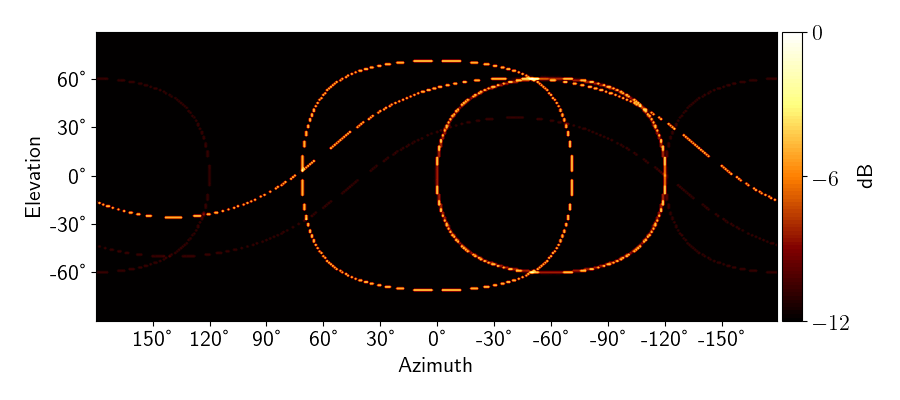
\includegraphics[width=0.8\textwidth]{Figures/2SrcNorm.png}
\end{subfigure}
\vskip \baselineskip
\begin{subfigure}[b]{0.96\textwidth}
    \centering
    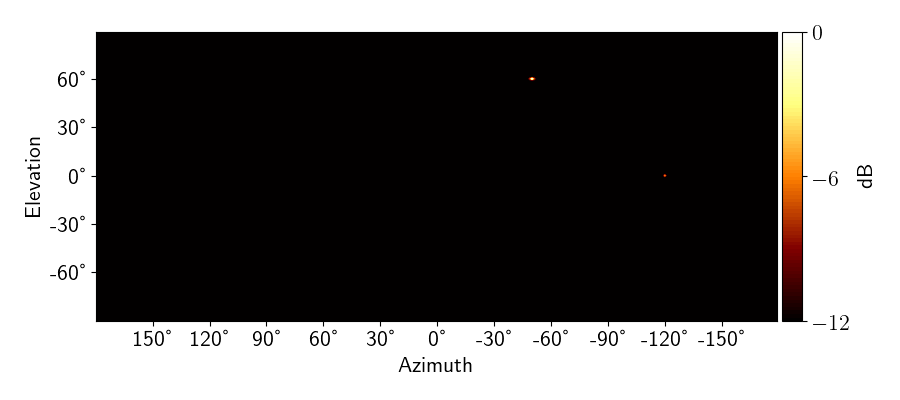
\includegraphics[width=0.8\textwidth]{Figures/2SrcMin.png}
\end{subfigure}
\caption{Figures depict localization results for sources at $(-50\degree,60\degree)$ having magnitude 0 dB and $(-120\degree,0\degree)$ having magnitude -6 dB, for normal SRP-PHAT (top) and minimum power SRP-PHAT (bottom). In normal SRP-PHAT, power from the source at $(-50\degree,60\degree)$ affects the result for the source at $(-120\degree,0\degree)$ since they share a localization circle. Minimum-power SRP handles this issue, since the minimum power cone at $(-120\degree,0\degree)$ is that of $(-120\degree,0\degree)$, thus the higher magnitude result from $(-50\degree,60\degree)$ is rejected.}
\label{fig:2srcsSameCone}
\end{figure}
Image sources due to reflection will also have the incorrect power for normal SRP-PHAT due to the same reason. The image source power will increase the main source power and vice versa, as they share two localization circles for a horizontal tetrahedral array. Minimum power SRP-PHAT automatically takes care of the errors due to reflection (discussed later in Fig. \ref{fig:4mic1srcRef}). \\

With minimum power SRP-PHAT, the redundant pair information would always improve results in low SNR conditions. This is because only the lowest power from all possible microphone pairs are used. The redundant pair information will thus result in removal or lowering of results in the non-source positions caused by noise. Fig. \ref{fig:minSRPDep} describes this affect. 
\begin{figure}[!ht]
    \centering
    \begin{subfigure}[b]{0.96\textwidth}
    \centering
    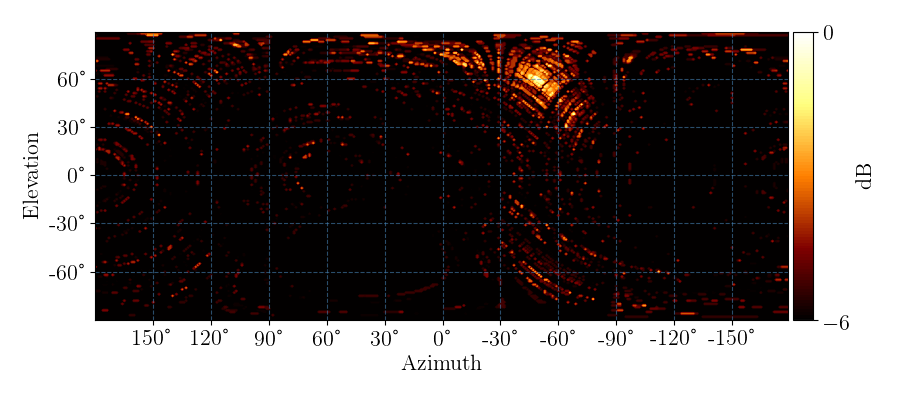
\includegraphics[width=0.8\textwidth]{Figures/Ind4mic1srcMinPowNeg6LowDyn.png}
\end{subfigure}
\vskip \baselineskip
\begin{subfigure}[b]{0.96\textwidth}
    \centering
    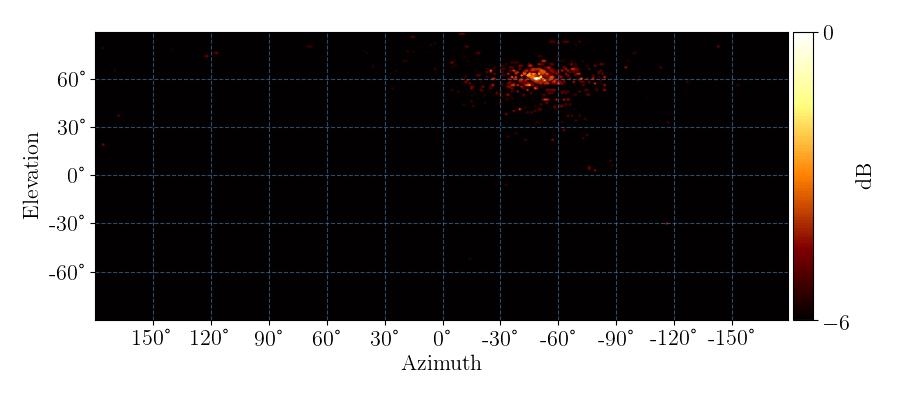
\includegraphics[width=0.8\textwidth]{Figures/Dep4mic1srcMinPowNeg6LowDyn.png}
\end{subfigure}
\caption{Figures depict localization results for source at $(50\degree,60\degree)$ for minimum power SRP-PHAT with only independent microphone pairs (top) and minimum power SRP-PHAT with all microphone pairs (bottom). As expected, using all microphone pairs results in removal of some of the incorrect results from the independent microphone pairs (To highlight the differences, the SNR for this simulation is kept at -6dB and the dynamic range has been reduced to 6dB).}
\label{fig:minSRPDep}
\end{figure}
\subsection{Multi-source localization}
As can be seen in fig. \ref{fig:4mic1srcInd}, even in ideal conditions, the localization results from SRP-PHAT contain many peaks of varying heights. This is due to summing the cross-correlation responses of a non-linear array (Eq. \ref{eq:srpSumInd}). If the array was linear, the localization circles from each pair would all overlap completely. In case of a tetrahedral array, the localization circles from the possible microphone pairs are not co-planar. This is because all the edges of a tetrahedron point in the different directions. The obvious problem here is the unpredictable behavior of the algorithm when multi-source are present. When multiple sources are playing at different levels, a detected peak can either be a real source or a pseudo-source created by an other higher level source. Methods are investigated to resolve the ambiguity between real source and the microphone array response. The methods to do so form the basis of deconvolution methods for SRP-PHAT.
\subsection{Source level retrieval}\label{srcLvlRetrieval}
For outdoor sound map reconstruction, the actual magnitude of the different outdoor sources is required. PHAT normalization essentially whitens the power signal, so the actual magnitude cannot be retrieved from the SRP-PHAT algorithm. However, the relative power levels between sources are maintained during SRP-PHAT\footnote{Errors can exist in normal SRP-PHAT, if two sources share localization cones. This can be due to the sources being located on the same cone of one or more microphone pairs. This can also occur during reflection, when if the tetrahedral array is placed horizontally, 3 cones out of 6 will always be shared between the source and the reflection.}.  
This can be utilized to retrieve the required levels. Various studies have been made on the correctness of the source power computed in this manner. In one study, the author compares the error in multi-source power, when instead of summing the SRP-PHAT as is done for normal SRP-PHAT, the powers are computed using geometric (GM) and harmonic means (HM) \cite{padois2016use}. As GM and HM give, by their nature, more weight to the lower values, doing GM and HM is essentially moving towards a minimum power SRP-PHAT approach. 
Suppose, the total measured magnitude is $E_{tot}$ Pa and M point sources produce $e_i$ $(i=1,2,....M)$ at the microphone array respectively\footnote{assuming far-field so that all microphones receive the same level from the same source}. Then, 
\begin{equation}
E_{tot}=\sum\limits_{i=1}^{M}e_i,
\end{equation}
suppose also, that the total measured volts by the microphones in the array is $V_{tot}$. We have:
\begin{equation}
    \frac{V_{tot}}{E_{tot}} = S,
\end{equation}
where S (V/Pa) is the sensitivity for the microphones in the array. Now, the information retrieved by the SRP-PHAT is a normalized digital value. This is retrieved for each point of the SRP search, i.e. (360*180) points if the search is done at a $1\degree$ resolution. Now, let the computed digital values for the sources be $d_i$ respectively, then,
\begin{equation}
    \frac{d_i}{e_i} = \frac{D_{tot}}{E_{tot}}, 
\end{equation}
we have,
\begin{equation}\label{eq:srcLvl}
\begin{split}
    e_i &= \frac{d_i\cdot E_{tot}}{D_{tot}} \\
        &= \frac{d_i}{D_{tot}} * \frac{V_{tot}}{S},
\end{split}
\end{equation}
The value from $\frac{d_i}{D_{tot}}$ is retrieved from the SRP-PHAT algorithm. $V_{tot}$ is measured during the experiments. Then, if S is known, the energy from each source can be computed. 
\subsection{Pre-processing}

Pre-processing the outdoor recordings before running SRP-PHAT is discussed in this section. Filtering the recorded signal can be extremely usefull to isolate certain frequencies of the signal as well as unmasking source with a different frequency content or different level for exemple a low frequency rumbling from speech signals. For outdoor source localization, lower frequencies are interesting as they can propagate further in the atmosphere \footnote{(Appendix \ref{app_outdoor}, Sec. \ref{app_atmabs})} while they can also be difficult to localize due to their large wavelengths\footnote{The phase difference, between the waveform received by a pair of microphone separated in space, depends on the distance of separation as well as the frequency of the waveform. Low frequency waves will have lesser phase difference.}, higher frequencies can be difficult due to aliasing\footnote{If more than one wavelength can fit between the two microphones, the cross-correlation peak delay will be ambiguous as it will become periodic.}. Cross-spectrum techniques are great to compute the cross correlation efficiently however it requires a long recording time to obtain a good  cross correlation dynamic range between the signal and the noise. This is critical to use a long acquisition time to lower the noise floor and to average out the random unexpected signal from the cross correlation\footnote{Stationary signal need time to build up in the cross-spectrum}. Therefore it might be necessary to filter out the noise from the signal when the acquisition time is small. Regarding high frequencies, if aliasing happens, the peaks in the cross-correlation of each microphones pair will be periodic however since each linearly independent pair of microphones will experience different time delays, the periodic peaks in the cross-correlation will be removed when taking the minimum power. A more limiting factor for high frequencies could actually be the phase matching of the microphones, as the frequency get higher, it is hard to notice phase differences \footnote{$+/- 5\degree$ from 3000 to 5000 Hz with B\&K type 4935}. Frequency filtering the signal to remove frequency bands where the signal is affected by noise or other distortions such as spatial aliasing appears to be a good idea however there are some implication on the processing delay. Some filtering techniques alter the phase or introduce pre-ringing in the signal therefore the filtering technique is critical. The min-power SRP-PHAT algorithm use the PHAT transform, which whiten the magnitude of the signal in order to only use the phase information to localize. For this reason a zero-phase filter is considered in our specific case where causality is not an issue but a linear-phase filter could also be used \footnote{Linear phase filters introduce processing delay but are causal}. Filtering out the spectrum proved really usefull in separating sources and results can be found in section blabla and appendix. Details on the implementation of the filter can be found in appendix \ref{app:filterdesign}. FFT filtering could potentially be very efficient to implement in the min-power SRP-PHAT however it introduces phase issues, also high order filter are used in this case therefore low order linear-phase filter must be implemented in case of real-time implementation, this requires more research on how to design a more efficient filtering technique minimizing distortions in the localization results. 

%First of all it has been discussed whether the files recorded must be filtered. Filtering is always a trade-off, in order to completely remove some frequency bands sharp filters are needed. While this is interesting for looking at different frequencies, it more or less transform our broadband algorithm into a narrow-band one. 
%The min-power SRP-PHAT is looking at localizing the stationary sound sources in the far field. Indeed the cross-correlation if taken over large time windows while discard the sources that are not stationary i.e that appear as random noise in the signal. Therefore it is clear that by taking large windows, the stationary sources are going to peak higher in the cross correlation, also a higher dynamic range can be achieved. Figures \ref{fig:avoir} display the result of a real-life measurement with different file length.

%\begin{figure}[H]
%    \centering
%    \begin{subfigure}[b]{0.8\textwidth}
%    \centering
%    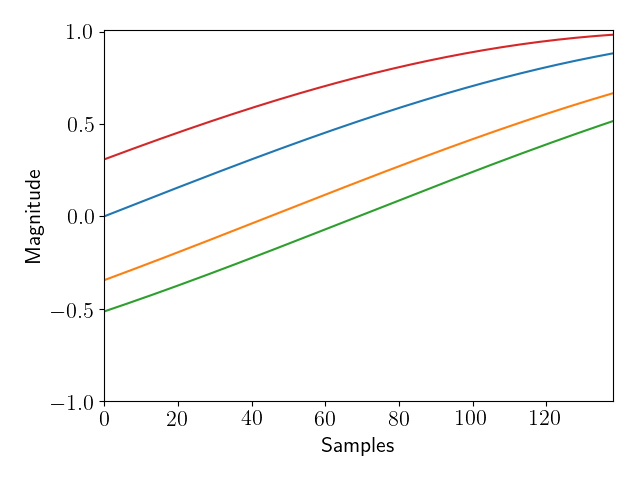
\includegraphics[width=0.8\textwidth]{Figures/60hz.png}
%    \end{subfigure}
%    \vskip \baselineskip
%    \begin{subfigure}[b]{0.8\textwidth}
%    \centering
%    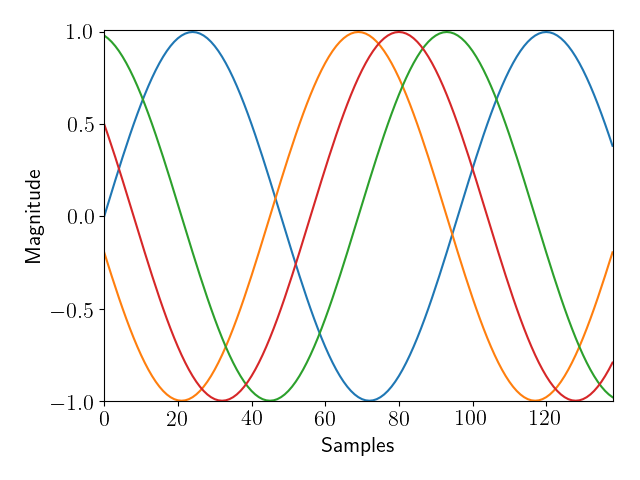
\includegraphics[width=0.8\textwidth]{Figures/500hz.png}
%    \end{subfigure}
%    \caption{Sine waves received at some time t on a 1m tetrahedral microphone array at 60Hz(top) and 500Hz(bottom)}
%    \label{fig:sineWavRec}
%\end{figure}

